\documentclass[10pt,a4paper]{article}
\usepackage{booktabs}
\usepackage[utf8]{inputenc}
\usepackage[T1]{fontenc}
\usepackage[spanish, es-tabla]{babel}
\usepackage{amsmath, amsfonts, amssymb, amsthm}
\usepackage{graphicx}
\usepackage[left=2.54cm, right=2.54cm, top=2.54cm, bottom=2.54cm]{geometry}
\usepackage{tikz}
\usepackage{soul}
\usepackage{listings}
\usepackage[most]{tcolorbox}
\usepackage{float}
\tcbset{shield externalize}
\usetikzlibrary{arrows.meta, positioning, automata}
\usetikzlibrary{babel}
\usepackage{hyperref}

%--------------------------------------------------------------------------------

% Bloque de Ejercicio
\newtcbtheorem[number within=section]{ejercicio}{Ejercicio}{
    enhanced,
    sharp corners,
    boxrule=0pt,
    leftrule=5pt,
    colframe=gray!30!black,
    colback=gray!5!white,
    coltitle=white,
    fonttitle=\bfseries,
    separator sign={.\ },
    before skip=10pt,
    after skip=10pt
}{ej}

% Bloque de Teoremas
\newtcbtheorem[number within=section]{mytheo}{Teorema}{
    enhanced,
    sharp corners,
    boxrule=0pt,
    leftrule=5pt,
    colframe=blue!40!black,
    colback=blue!5!white,
    coltitle=white,
    fonttitle=\bfseries,
    separator sign={.\ },
    before skip=10pt,
    after skip=10pt
}{th}

 % Bloque de Alerta
\newtcolorbox{alerta}[1]{
    enhanced,
    sharp corners,
    boxrule=0pt,
    leftrule=5pt,
    colframe=red!40!black,
    colback=red!5!white,
    coltitle=white,
    fonttitle=\bfseries,
    title=#1,
    before skip=10pt,
    after skip=10pt
}

% Bloque de Notas
\newtcolorbox{nota}[1]{
    enhanced,
    sharp corners,
    boxrule=0pt,
    leftrule=5pt,
    colframe=orange!40!black,
    colback=yellow!5!white,
    coltitle=white,
    fonttitle=\bfseries,
    title=#1,
    before skip=10pt,
    after skip=10pt
}

% ---------------------------------------------------------------------------------------------
\begin{document}

\begin{titlepage}
    \centering
    {\huge \textbf{Universidad Nacional Autónoma de México}}\\[0.3cm]
    \rule{\linewidth}{2mm}\\[0.3cm]
    {\large \textbf{Facultad de Estudios Superiores Acatlán}}\\[1cm]
    

    
\includegraphics[width=6cm]{../../Archivos/Imagenes_Logos/acatlan.png}\\[1cm]
    
    {\Large \textbf{Matemáticas Aplicadas y Computación}}\\[1cm]
    {\huge \textit{Optimización 2}}\\[0.5cm]
    \rule{\linewidth}{0.3mm}\\[0.3cm]
    {\Large \textit{Programación Entera y Método Gráfico}}\\[0.3cm]
    \rule{\linewidth}{0.3mm}\\[0.3cm]
    
    \vfill
    
    \rule{\linewidth}{0.5mm}\\[0.3cm]
    {\Large \textit{Ricardo López Ramírez}}\\
    \rule{\linewidth}{0.5mm}\\[0.8cm]
    
 \small
    Actualización: \today \hfill Página: \thepage
\end{titlepage}

% ÍNDICE 
\pagenumbering{roman}
\tableofcontents
\cleardoublepage
\pagenumbering{arabic}
\setcounter{page}{1}

% CONTENIDO 
\section{Programas de Programación Entera y Método Gráfico.}


\begin{ejercicio}{1. Investigación de herramientas de cómputo}{ej1}
Investigar 4 diferentes herramientas de cómputo, chatgpt o en su caso apps de programación entera y llena, incluye al menos tres características:
\end{ejercicio}

\vspace{0.4cm}
Herramientas computacionales altamente relevantes para el modelado, 
resolución e interpretación de problemas de Programación Entera y Método Gráfico.

\begin{center}
\renewcommand{\arraystretch}{1.6} 
\begin{tabular}{p{3.5cm} p{4.5cm} p{7cm}}
\toprule
\textbf{Herramienta} & \textbf{Url o APP} & \textbf{Características de la herramienta} \\
\midrule

\textbf{1. Python} \newline (Librería PuLP / Gurobipy) & 
\url{https://pypi.org/project/PuLP/} & 
$\bullet$ Interfaz de código abierto para modelar problemas de optimización usando sintaxis de programación pura.\newline
$\bullet$ Permite integrar e invocar potentes \textit{solvers} comerciales y libres (CBC, GLPK, Gurobi, CPLEX).\newline
$\bullet$ Altamente escalable, ideal para el análisis de datos y la automatización de decisiones a gran escala.\\
\midrule

\textbf{2. LINGO} & 
\url{https://www.lindo.com/} & 
$\bullet$ Lenguaje de modelado matemático clásico y robusto, estándar en cursos de Investigación de Operaciones.\newline
$\bullet$ Su interfaz permite escribir las funciones objetivo y restricciones casi idénticas a la notación algebraica matemática.\newline
$\bullet$ Destaca por su capacidad para manejar variables enteras y binarias de forma nativa e integrarse con bases de datos.\\
\midrule

\textbf{3. GeoGebra} \newline (Para Método Gráfico) & 
\url{https://www.geogebra.org/calculator} & 
$\bullet$ Plataforma gráfica interactiva, ideal para resolver sistemas de dos variables mediante el Método Gráfico.\newline
$\bullet$ Permite graficar sistemas de inecuaciones para visualizar la región factible con un sombreado automático.\newline
$\bullet$ El uso de "deslizadores" permite animar la función objetivo ($Z$) para identificar visualmente los vértices óptimos.\\
\midrule

\textbf{4. Google Gemini} \newline (Asistente IA Multimodal) & 
\url{https://gemini.google.com/} & 
$\bullet$ Modelo de inteligencia artificial multimodal capaz de analizar imágenes de problemas de optimización y traducirlos a una formulación matemática rigurosa.\newline
$\bullet$ Genera código estructurado (Python, LINGO) a partir de modelos matemáticos y proporciona directamente la sintaxis en \LaTeX\ para reportes académicos.\newline
$\bullet$ Funciona como tutor interactivo, explicando paso a paso la lógica detrás de algoritmos complejos (Branch and Bound, Simplex) para validar resultados.\\
\bottomrule
\end{tabular}
\end{center}

\begin{nota}{Importancia en la Licenciatura en MAC}
La combinación de estas cuatro herramientas cubre el ciclo completo de la optimización: \textbf{Gemini} asiste en el planteamiento lógico y la redacción del modelo, \textbf{GeoGebra} proporciona la intuición geométrica en 2D, y \textbf{LINGO} o \textbf{Python} ejecutan el motor de cálculo riguroso para sistemas de Programación Entera Mixta multidimensionales.
\end{nota}

\newpage

\begin{ejercicio}{2. Resolución computacional de modelos}{ej2}
Elegir al menos una herramienta de las analizadas anteriormente y resolver los siguientes modelos:
\begin{enumerate}
    \item[a)] $\max z = 5x_1 + 2x_2$ \\
    s.a. \\
    $2x_1 + 2x_2 + x_3 = 9$ \\
    $3x_1 + x_2 + x_4 = 11$ \\
    $x_j \ge 0$ \\
    $x_j \in \mathbb{Z}$
    
    \item[b)] $\max z = 5x_1 + 2x_2$ \\
    s.a. \\
    $2x_1 + 2x_2 + x_3 = 9$ \\
    $3x_1 + x_2 + x_4 = 11$ \\
    $x_j \ge 0$ \\
    $x_2, x_4 \in \mathbb{Z}$
\end{enumerate}

\end{ejercicio}

\vspace{0.4cm}
\textbf{Herramienta computacional seleccionada:} Python (Librería PuLP).

A continuación, se presenta el código fuente utilizado para resolver ambos modelos, 
seguido de la interpretación de la salida del \textit{solver}. 
Esta herramienta nos permite definir la naturaleza exacta de cada variable 
(continua o entera).

\begin{lstlisting}[language=Python, frame=single, title={Resolución de Modelos en Python (PuLP)}]
import pulp
# Modelo A: Programacion Entera Pura (PIP)
prob_a = pulp.LpProblem("Modelo_A", pulp.LpMaximize)

# Definicion de variables (Todas enteras)
x1_a = pulp.LpVariable('x1', lowBound=0, cat='Integer')
x2_a = pulp.LpVariable('x2', lowBound=0, cat='Integer')
x3_a = pulp.LpVariable('x3', lowBound=0, cat='Integer')
x4_a = pulp.LpVariable('x4', lowBound=0, cat='Integer')

# Funcion Objetivo y Restricciones
prob_a += 5*x1_a + 2*x2_a, "Z"
prob_a += 2*x1_a + 2*x2_a + x3_a == 9
prob_a += 3*x1_a + x2_a + x4_a == 11
prob_a.solve()

# Modelo B: Programacion Entera Mixta (MIP)
prob_b = pulp.LpProblem("Modelo_B", pulp.LpMaximize)
# Definicion de variables (Mixtas)
x1_b = pulp.LpVariable('x1', lowBound=0, cat='Continuous')
x2_b = pulp.LpVariable('x2', lowBound=0, cat='Integer')
x3_b = pulp.LpVariable('x3', lowBound=0, cat='Continuous')
x4_b = pulp.LpVariable('x4', lowBound=0, cat='Integer')

# Funcion Objetivo y Restricciones
prob_b += 5*x1_b + 2*x2_b, "Z"
prob_b += 2*x1_b + 2*x2_b + x3_b == 9
prob_b += 3*x1_b + x2_b + x4_b == 11
prob_b.solve()
\end{lstlisting}

\begin{figure}[H]
    \centering
    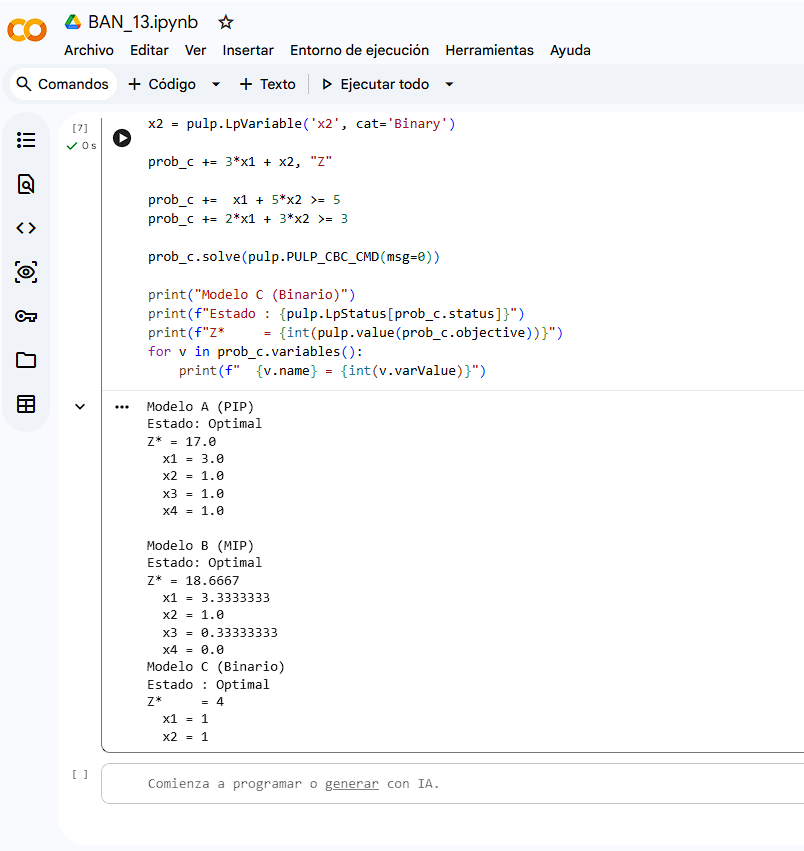
\includegraphics[width=0.6\linewidth]{../../Archivos/Imagenes_Logos/Codigo_BAN_13.png}
    \caption{Codigopy}
    {\small Enlace: \url{https://colab.research.google.com/drive/1v2ut-0B9BBSgz_9VnK1-DHakaIt7wxIC?usp=sharing}}
\end{figure}

\vspace{0.6cm}
\textbf{Interpretación de Resultados}

\textbf{Modelo a - Programación Entera Pura (PEP)}\\
En este modelo, se exige estrictamente que todas las variables ($x_1, x_2, x_3, x_4$) 
pertenezcan al conjunto de los números enteros ($\mathbb{Z}$). 
Tras ejecutar el algoritmo de Ramificación y Acotamiento, obtenemos la siguiente solución óptima:
\begin{itemize}
    \item $x_1 = 3$
    \item $x_2 = 1$
    \item Variables de holgura: $x_3 = 1$, $x_4 = 1$
    \item \textbf{Valor óptimo de la función objetivo:} $Z = 5(3) + 2(1) = 17$
\end{itemize}
\textit{Análisis:} Al ser un problema entero puro, el solver sacrifica parte de la región factible continua para anclarse en la coordenada entera más rentable. Ambas restricciones se cumplen perfectamente ($2(3) + 2(1) + 1 = 9$ y $3(3) + 1 + 1 = 11$).

\vspace{0.4cm}
\textbf{Modelo b- Programación Entera Mixta (PEM)}\\
En este modelo se relaja la restricción de integralidad para $x_1$ y $x_3$, permitiendo que asuman valores fraccionarios (continuos), mientras que $x_2$ y $x_4$ siguen obligadas a ser enteras. La ejecución del solver arroja la siguiente solución óptima:
\begin{itemize}
    \item $x_1 = 3.333$ (Equivalente a la fracción $\frac{10}{3}$)
    \item $x_2 = 1$
    \item Variables de holgura: $x_3 = 0.333$ ($\frac{1}{3}$), $x_4 = 0$
    \item \textbf{Valor óptimo de la función objetivo:} $Z = 5(\frac{10}{3}) + 2(1) = \frac{56}{3} \approx 18.666$
\end{itemize}
\textit{Análisis:} Al permitir que $x_1$ sea continua, el modelo puede "estirar" el valor de esta variable para obtener una mayor rentabilidad en la función objetivo (pasa de $Z=17$ a $Z=18.666$). La variable $x_4 = 0$ (entera) obliga a que la segunda restricción se sature ($3x_1 + x_2 = 11$), lo cual es matemáticamente consistente con $3(\frac{10}{3}) + 1 = 11$.

\vspace{0.4cm}
\textbf{Modelo c) - Programación Entera Binaria}\\
Este modelo introduce una condición estricta: las variables solo pueden tomar el valor de 0 o 1 (decisiones dicotómicas de "sí" o "no"). La herramienta procesa las cuatro combinaciones posibles $(0,0), (0,1), (1,0), (1,1)$ y arroja la siguiente solución óptima:
\begin{itemize}
    \item $x_1 = 1$
    \item $x_2 = 1$
    \item \textbf{Valor óptimo de la función objetivo:} $Z = 3(1) + 1(1) = 4$
\end{itemize}
\textit{Análisis:} Dado que las variables son binarias, evaluamos la factibilidad lógicamente. 
Si $x_2 = 0$, la primera restricción ($x_1 \ge 5$) sería imposible de cumplir ya que 
$x_1$ máximo puede valer 1. Por lo tanto, el solver deduce inmediatamente que $x_2$ debe ser 
obligatoriamente $1$. Con $x_2=1$, ambas restricciones se 
cumplen ($1 + 5(1) \ge 5$ y $2x_1 + 3(1) \ge 3$). Como buscamos maximizar, 
el solver asigna $x_1 = 1$ para obtener el máximo beneficio posible, logrando $Z=4$ y 
satisfaciendo holgadamente ambas inecuaciones ($6 \ge 5$ y $5 \ge 3$).

\newpage

\begin{ejercicio}{Resolución mediante método gráfico a mano}{ej3}
Resolver los siguientes modelos usando el método gráfico. 
Se presentará la región factible continua y el proceso deductivo para localizar la solución óptima de acuerdo a la naturaleza de las variables (Enteras, Mixtas o Binarias).
\end{ejercicio}


% MODELO A

\vspace{0.4cm}
\textbf{\large a) Modelo de Programación Entera Mixta (PEM)}
\begin{align*}
    \text{Maximizar } Z &= 5x_1 + 4x_2 \\
    \text{s.a.} \quad 
    6x_1 + 4x_2 &\le 24 \quad \text{(L1)} \\
    x_1 + 2x_2 &\le 7 \quad \text{(L2)} \\
    -x_1 + x_2 &\le 1 \quad \text{(L3)} \\
    x_2 &\le 2 \quad \text{(L4)} \\
    x_1, x_2 &\ge 0 \\
    x_2 &\in \mathbb{Z} \quad (x_1 \text{ es continua})
\end{align*}

\textbf{Graficar la región continua.} Se trazan las rectas asumiendo que ambas variables son 
continuas.
\begin{itemize}
    \item L1 cruza en $(0, 6)$ y $(4, 0)$.
    \item L2 cruza en $(0, 3.5)$ y $(7, 0)$.
    \item L3 cruza en $(0, 1)$ y $(-1, 0)$.
    \item L4 es una recta horizontal en $x_2 = 2$.
\end{itemize}

\textbf{Aplicar la restricción mixta.} Como $x_2$ debe ser entera y está acotada 
por $0 \le x_2 \le 2$, la región factible real no es un polígono, 
sino \textbf{tres segmentos de recta horizontales} 
ubicados en $x_2 = 0$, $x_2 = 1$ y $x_2 = 2$.

\begin{center}
\begin{tikzpicture}[scale=1.5]
    % Cuadrícula y Ejes
    \draw[help lines, step=1, gray!40] (-0.5,-0.5) grid (4.5,3.5);
    \draw[->, thick] (-0.5,0) -- (4.5,0) node[right] {$x_1$};
    \draw[->, thick] (0,-0.5) -- (0,3.5) node[above] {$x_2$};
    
    % Recorte para que las líneas no se salgan del gráfico
    \clip (-0.5,-0.5) rectangle (4.5,3.5);
    
    % Restricciones continuas (Líneas transparentes)
    \draw[red, thick, dashed] (0,6) -- (4,0) node[midway, sloped, above] {$L1$};
    \draw[blue, thick, dashed] (0,3.5) -- (7,0) node[midway, sloped, above] {$L2$};
    \draw[green!60!black, thick, dashed] (-1,0) -- (2.5,3.5) node[midway, sloped, above] {$L3$};
    \draw[orange, thick, dashed] (-0.5,2) -- (4.5,2) node[pos=0.1, above] {$L4$};

    % Segmentos factibles mixtos (x2 entera)
    \draw[ultra thick, purple] (0,0) -- (4,0) node[right] {$x_2=0$};
    \draw[ultra thick, purple] (0,1) -- (3.333,1) node[right] {$x_2=1$};
    \draw[ultra thick, purple] (1,2) -- (2.666,2) node[above left] {$x_2=2$};
    
    % Puntos extremos de los segmentos a evaluar
    \fill[black] (4,0) circle (2pt);
    \fill[black] (3.333,1) circle (2pt);
    \fill[purple] (2.666,2) circle (3pt) node[above right] {\textbf{Óptimo $(8/3, 2)$}};
\end{tikzpicture}
\end{center}

\textbf{Evaluación de vértices mixtos.} Evaluamos $Z = 5x_1 + 4x_2$ en los 
extremos derechos de cada segmento factible (ya que buscamos maximizar):
\begin{itemize}
    \item Para $x_2 = 0$, el límite lo dicta L1: $6x_1 \le 24 \implies x_1 = 4$. Pto $(4, 0) \rightarrow Z = 20$
    \item Para $x_2 = 1$, el límite lo dicta L1: $6x_1 + 4 \le 24 \implies x_1 = 10/3$. Pto $(10/3, 1) \rightarrow Z = 5(10/3) + 4 = 20.66$
    \item Para $x_2 = 2$, el límite inferior lo da L3 ($-x_1+2 \le 1 \implies x_1 \ge 1$) y el superior lo da L1 ($6x_1 + 8 \le 24 \implies x_1 = 8/3$). Pto $(8/3, 2) \rightarrow Z = 5(8/3) + 8 = \mathbf{21.33}$
\end{itemize}
\textbf{Solución Óptima:} $x_1 = 8/3$, $x_2 = 2$, con $Z = 64/3 \approx 21.33$.


% MODELO B
\vspace{0.8cm}
\textbf{\large b) Modelo de Programación Entera Binaria}
\begin{align*}
    \text{Minimizar } Z &= x_1 + 3x_2 \\
    \text{s.a.} \quad 
    x_1 + x_2 &\ge 2 \quad \text{(L1)} \\
    x_1 - 3x_2 &\le 2 \quad \text{(L2)} \\
    x_1 - x_2 &\le 1 \quad \text{(L3)} \\
    -x_1 + x_2 &\le 1 \quad \text{(L4)} \\
    x_1, x_2 &\in \{0, 1\}
\end{align*}

\textbf{Análisis del dominio binario.} Al ser un problema binario, 
el espacio de soluciones posibles se reduce exclusivamente a 4 puntos discretos:
 $(0,0), (0,1), (1,0), \text{y } (1,1)$. 

\textbf{Prueba de factibilidad gráfica.} Solo necesitamos graficar la primera restricción ($L1: x_1 + x_2 \ge 2$) para darnos cuenta del comportamiento del modelo.

\begin{center}
\begin{tikzpicture}[scale=2]
    % Cuadrícula y Ejes
    \draw[help lines, step=1, gray!50] (-0.5,-0.5) grid (1.5,1.5);
    \draw[->, thick] (-0.5,0) -- (1.5,0) node[right] {$x_1$};
    \draw[->, thick] (0,-0.5) -- (0,1.5) node[above] {$x_2$};
    
    % Puntos binarios
    \fill[gray] (0,0) circle (2pt) node[below left] {$(0,0)$ Inviable};
    \fill[gray] (1,0) circle (2pt) node[below right] {$(1,0)$ Inviable};
    \fill[gray] (0,1) circle (2pt) node[above left] {$(0,1)$ Inviable};
    
    % Restricción crítica
    \draw[red, thick, dashed] (-0.5, 2.5) -- (2.5, -0.5) node[midway, sloped, above] {$x_1 + x_2 \ge 2$};
    \fill[blue!10, opacity=0.5] (0,2) -- (2,0) -- (2,2) -- cycle;
    
    % Óptimo
    \fill[purple] (1,1) circle (3pt) node[above right] {\textbf{Único factible $(1,1)$}};
\end{tikzpicture}
\end{center}

\textbf{Evaluación.} La restricción L1 exige que la suma de las variables sea al menos 2. De las 4 coordenadas binarias, la única que logra esto matemáticamente es $(1,1)$. Procedemos a verificar el resto de restricciones para este único punto:
\begin{itemize}
    \item L2: $1 - 3(1) = -2 \le 2$ (Cumple)
    \item L3: $1 - 1 = 0 \le 1$ (Cumple)
    \item L4: $-1 + 1 = 0 \le 1$ (Cumple)
\end{itemize}
Al existir solo un punto factible en todo el espacio vectorial, este se convierte automáticamente en el óptimo, sin importar si buscamos maximizar o minimizar. \\
\textbf{Solución Óptima:} $x_1 = 1$, $x_2 = 1$, con $Z = 1 + 3(1) = \mathbf{4}$.


% MODELO C

\vspace{0.8cm}
\textbf{\large c) Modelo de Programación Entera Pura (PEP)}
\begin{align*}
    \text{Maximizar } Z &= 4x_1 + 6x_2 \\
    \text{s.a.} \quad 
    2x_1 + 3x_2 &\le 6 \quad \text{(L1)} \\
    6x_1 + 4x_2 &\le 12 \quad \text{(L2)} \\
    -2x_1 + 2x_2 &\le 2 \implies -x_1 + x_2 \le 1 \quad \text{(L3, simplificada)} \\
    x_1 + x_2 &\ge 2 \quad \text{(L4)} \\
    x_1, x_2 &\ge 0 \\
    x_1, x_2 &\in \mathbb{Z}
\end{align*}

\textbf{Delimitar} 
La intersección de $L1$ (que pasa por $(0,2)$ y $(3,0)$) y $L4$ (que pasa por $(0,2)$ y $(2,0)$) forma un triángulo estrecho.
Resolviendo el sistema entre $L1$ y $L2$, el vértice más lejano del origen ocurre en el punto fraccionario $(1.2, 1.2)$.

\textbf{Identificar los puntos enteros interiores.} Superponemos la cuadrícula entera sobre la región factible continua sombreada.

\begin{center}
\begin{tikzpicture}[scale=2]
    % Cuadrícula y Ejes
    \draw[help lines, step=1, gray!40] (-0.5,-0.5) grid (3.5,2.5);
    \draw[->, thick] (-0.5,0) -- (3.5,0) node[right] {$x_1$};
    \draw[->, thick] (0,-0.5) -- (0,2.5) node[above] {$x_2$};
    
    \clip (-0.5,-0.5) rectangle (3.5,2.5);
    
    % Región factible continua
    \fill[blue!15] (0,2) -- (1.2,1.2) -- (2,0) -- cycle;
    
    % Restricciones
    \draw[red, thick] (0,2) -- (3,0) node[pos=0.8, above right] {$L1$}; 
    \draw[blue, thick] (0,3) -- (2,0) node[pos=0.8, right] {$L2$};
    \draw[green!60!black, thick] (0,2) -- (2,0) node[pos=0.5, below left] {$L4$};
    
    % Puntos enteros evaluados
    \fill[black] (2,0) circle (2pt) node[below right] {$(2,0)$};
    \fill[black] (1,1) circle (2pt) node[below left] {$(1,1)$};
    \fill[purple] (0,2) circle (3pt) node[above right] {\textbf{Óptimo $(0,2)$}};
\end{tikzpicture}
\end{center}

\textbf{Evaluación de coordenadas.} Los únicos tres puntos cuyas coordenadas $x_1$ y $x_2$ son números enteros exactos y que caen dentro o sobre las fronteras del área sombreada son $(0,2)$, $(2,0)$ y $(1,1)$. Procedemos a evaluar $Z = 4x_1 + 6x_2$:
\begin{itemize}
    \item Para $(2,0) \rightarrow Z = 4(2) + 6(0) = 8$
    \item Para $(1,1) \rightarrow Z = 4(1) + 6(1) = 10$
    \item Para $(0,2) \rightarrow Z = 4(0) + 6(2) = 12$
\end{itemize}
\textbf{Solución Óptima:} El punto que maximiza la utilidad respetando la condición de integralidad es $x_1 = 0$, $x_2 = 2$, con un valor $Z = \mathbf{12}$.


\end{document}